\chapter{Formal background}

In this chapter, we introduce the concept of planning to help us  formalize the studied transportation problems.

\section{Automated planning}

As previously stated, \textit{planning} is usually defined as the reasoning side of acting --- an abstract deliberation
process that chooses and organizes actions by anticipating their outcomes. \citep[Section~1.1]{Ghallab2004}
It seems only natural that we want to have computers do this strenuous activity for us.
Automated planning is an attempt at just that --- it is an area of Artificial Intelligence (AI) that
studies the planning process computationally. \citep[Section~1.1]{Ghallab2004}

Unfortunately, the specific situations in which we want to use automated planning are very diverse
--- from devising a sequence of actions to shut down a nuclear power plant,
planning the movements of a robotic arm
on an assembly line, or devising the complex pattern of motor activations
for space aircraft positioning.
Due to this, researchers are often interested in domain-independent planning,
where the planner gets information
about both the domain and the specific problem at runtime and attempts to devise a plan using only the provided knowledge
and the planner's previously built-in processes. \citep[Section~1.3]{Ghallab2004}

On the other hand, domain-specific planning, where domain knowledge has been built into the planner,
has obvious advantages when solving problems in that domain --- all the while being useless on problems of other
domains. \citep[Section~1.3]{Ghallab2004}

\section{Planning model}

As a basis for the later-defined representation of planning, we first define
a conceptual model similar to the restricted model in \citep[Section~1.4, Section~1.5]{Ghallab2004}.

\begin{defn}[State-transition system]\label{defn:state-transition-sys}
A (restricted) state-transition system is a 3-tuple $\Sigma = (S, A, \gamma)$, where:
\begin{itemize}
\item $S = \{s_1, s_2, \ldots\}$ is a finite and fully observable set of states;
\item $A = \{\noop, a_1, a_2, \ldots\}$ is a finite set of actions;
\item $\gamma: S \times A \to S \cup \{\emptyset\}$ is a state-transition function,
where $\forall s \in S : \gamma(s, \noop) = s$; and
\item $\Sigma$ is static and offline,
it only changes when an action is applied to it and does not change while planning.
\end{itemize}
In the basic version, all actions have no duration.
\end{defn}

For a state $s \in S$, the actions $A_s = \{a \in A | \gamma(s, a) \neq \emptyset\}$ are called \textit{applicable}
to the given state $s$. The $\noop$ action is applicable to all states.

The state-transition function $\gamma$ and the set of actions $A$ together loosely correspond to what we will call a \textit{planning domain}.
Planning domains define an abstract representation of actions we work with
and how they are related,
but they do not state anything about specific states or actions.

Given a state-transition system $\Sigma$, planning aims to find a
sequence of actions to apply to the initial state in order to achieve some objective.
The objective can be defined in various ways --- we might want the planner
to devise a plan that
does not enter specific states, or contrary to that, visits each of a set of states,
or one that just ends at a chosen state.
We will use the last option for formalizing the notion of a \textit{planning problem}.

\begin{defn}[Planning problem]\label{defn:planning-problem}\citep[Part~I]{Ghallab2004}
A planning problem is a 5-tuple $\mathcal{P} = (S, A, \gamma, s_0, g)$, where:
\begin{itemize}
\item $(S, A, \gamma)$ is a state-transition system;
\item $s_0 \in S$ is an initial state; and
\item $g \subseteq S$ is a set of goal states.
\end{itemize}
\end{defn}

Now that we have defined a \textit{planning problem} we can specify what we mean
by the planner generating a \textit{sequence of actions} to achieve a goal --- we will
call this sequence a \textit{plan}.

\begin{defn}[Plan]\label{defn:plan}\citep[Section~1.5]{Ghallab2004}
For a planning problem $\mathcal{P} = (S, A, \gamma, s_0, g)$,
a plan is a finite sequence of actions $(a_1, a_2, \ldots, a_k),\, k \in \N$ where
$\forall i \in \kset : a_i \in A$ and
$\forall i \in \kset : \gamma(s_{i-1}, a_i) = s_i \in S$, while $s_k \in g$.
\end{defn}

A basic \textit{planning model}, i.e. the abstraction of a whole real-life scenario
we want to plan for, consists of three components (Figure~\ref{fig:planning-model}):
\begin{itemize}
\item A \textit{state-transition system} $\Sigma$, that evolves by using its state-transition function on the actions
it receives;
\item A \textit{controller}, that given an input state $s \in S$ and a generated plan, provides an action $a \in A$ as output; and
\item A \textit{planner}, that uses a description of the state-transition system $\Sigma$ to synthesize a plan for the controller
to execute in order to reach a goal state from the initial state.
\end{itemize}

\begin{figure}[tb]
\begin{center}
\includegraphics[width=0.7\textwidth]{../imga/planning_model}
\end{center}
\caption[A typical planning model for offline planning.]{A typical planning model for offline planning --- a state-transition system $\Sigma$, a controller executing a plan, and a planner devising the plan based on an initial state and goals. Adapted from \citep[Figure~1.3]{Ghallab2004}.}
\label{fig:planning-model}
\end{figure}

\section{Classical planning}\label{classical-planning}

Although the previously defined restricted state-transition system is a simplification of real-world
domains, it is a useful one. 
This simplification has historically been studied as classical planning.

A different branch of automated planning, \textit{neoclassical planning},
uses largely the same theoretical foundations as classical 
planning. What is different is the approach to planning using those foundations
--- instead of search space nodes being a sequence of actions or a partially ordered
set of actions, we view them as a set of several partial plans
\citep[Part~II]{Ghallab2004}.
One of the most famous results in neoclassical planning is the GraphPlan algorithm
published by \citet{Blum1997}. It is out of the scope of this text to describe it in detail
--- see \citet[Section~6.3]{Ghallab2004}.
GraphPlan makes heavy use of a data structure called a \textit{planning graph},
which caused a breakthrough in the field of (domain-independent) planning
--- bigger problems could now be practically solved.

We will now describe several theoretical domain-independent representations
of planning problems used in classical planning \citep[Chapter~2]{Ghallab2004},
so that we can formulate our domain using them.

\subsection{Set-theoretic representation}

Leveraging propositional logic, both the planning domain and problem
are represented with the notion
of proposition symbols $L = \{p_1, p_2, \ldots\}$.
Each state is defined as a subset of propositions of $L$ --- those propositions
which hold in the given state. $S$ is closed under the application of each
action $a \in A$.

An action $a$
is a triple of sets of propositions of $L$.
We denote the sets $a = (\precond(a), \effects^-(a), \effects^+(a))$, where:
\begin{itemize}
\item $\precond(a)$ are the \textit{preconditions} of an action: the set of
propositions that must hold in the current state for the action to be applicable to it;
\item $\effects^-(a)$ are the \textit{negative effects} of an action:
the set of propositions
that will no longer hold in the state once the action is applied; and
\item similarly, $\effects^+(a)$ are the \textit{positive effects} of an action:
the set of propositions that will be true in the state once the action is applied.
\end{itemize}
Note that an action cannot have the same proposition as a negative and positive effect at the same time --- the sets $\effects^+(a)$ and $\effects^-(a)$ are disjunct for all actions $a$.
The state-transition function is $\gamma(s, a) = (s - \effects^-(a)) \,\cup\,
\effects^+(a)$ if $a$ is applicable to $s$,
otherwise $\gamma(s, a)$ is undefined. Goal states $S_g$ are defined as
$S_g = \{s \in S \,|\, g \subseteq s\}$, where
$g \subseteq L$ is any chosen set of propositions. The propositions $g$ are called
\textit{goal propositions}.

\subsection{Classical representation}

The classical representation generalizes the set-theoretic representation using first-order logic,
without functions.
States are sets of ground atoms of a first-order language.
Actions are ground instances of \textit{planning operators},
triples $o = (\name(o), \precond(o), \effects(o))$:

\begin{itemize}
\item $\name(o)$ is a syntactic expression of the given operator;
\item $\precond(o)$ and $\effects(o)$ are sets of literals
(atoms and their negations), similar in use to their equivalents
in the set-theoretic case.
\end{itemize}
The definition of the state-transition function also stays the same.
Goal states are defined as the set of states that satisfy $g$,
the \textit{goal}, where $g$ is any set of ground literals.

The following is an example of a planning operator for driving a vehicle between two connected locations:
$$o_d = (\mt{drive}(v, f, t), \{\mt{at}(v, f), \mt{road}(f, t)\}, \{\mt{at}(v, t), \neg \mt{at}(v, f)\}).$$
The variable $v$ denotes a vehicle, $f$ and $t$ are the source and destination locations, respectively. The at predicate is true if and only if the vehicle is located at that position in the given state and the road predicate
is true if and only if a road exists between the two locations.
An example of an action instantiated from the operator (sometimes referred to as \textit{operator instance})
for a vehicle $\mt{v}_1$ and two locations $\mt{l}_1$ and $\mt{l}_2$ would be:
$$a_{\mt{drive}, \mt{v}_1, \mt{l}_1, \mt{l}_2} = (\mt{drive}(\mt{v}_1, \mt{l}_1, \mt{l}_2), \{\mt{at}(\mt{v}_1, \mt{l}_1),
\mt{road}(\mt{l}_1, \mt{l}_2)\}, \{\mt{at}(\mt{v}_1, \mt{l}_2), \neg \mt{at}(\mt{v}_1, \mt{l}_1)\}).$$


Both the set-theoretic and the classical representations follow the \textit{Closed world assumption} --- that any atom/predicate not present in the state does not hold in that state.

\subsection{State-variable representation}

The state-variable representation substitutes the use of relations of the previous
representation for functions,
using the concept of state variables. State variables are functions
that take the state as an input and serve as characteristic attributes, defining the state. We usually use a more practical way of defining these functions --- we assume
the current state as an input without denoting it, and instead add different inputs.

For example, a useful set of state-variable functions for a domain that contains a road
network and vehicles might be: $$\mathrm{location}_{v}: S \to \mathrm{locations},$$
where $v \in \mathrm{vehicles}$.
Instead, we could define a single function:
$$\mathrm{location'}: \mathrm{vehicles} \times S \to \mathrm{locations},$$
and afterwards 
$$\mathrm{location''}: \mathrm{vehicles} \to \mathrm{locations},$$
using $\mathrm{location''}(v) = \mathrm{location'}(v, state_{cur})$, where $state_{cur}$ is the current state.

Planning operators are defined similarly to the classical representation, but
$\precond(o)$ is now a set of expressions on state variables and relations.
Also, $\effects(o)$ is defined as a set of assignments of values to state variables.
For comparison, we show the same planning operator as in the classical representation:
$$o_d = \left(\mt{drive}(v, f, t), \{\mt{at}(v) = f, \mt{road}(f, t)\}, \{\mt{at}(v) \leftarrow t\}\right),$$
and an example of an action instantiated from this operator
for vehicle $\mt{v}_1$ and two locations $\mt{l}_1$ and $\mt{l}_2$:
$$a_{\mt{drive}, \mt{v}_1, \mt{l}_1, \mt{l}_2} = \left(\mt{drive}(\mt{v}_1, \mt{l}_1, \mt{l}_2), \{\mt{at}(\mt{v}_1) = \mt{l}_1,
\mt{road}(\mt{l}_1, \mt{l}_2)\}, \{\mt{at}(\mt{v}_1) \leftarrow \mt{l}_2\}\right).$$

The state-transition function is defined analogously to the classical representation: an action~$a$ (ground instance
of operator~$o$)
is applicable to a state~$s$ if the $\precond(o)$ condition is true given the values
of state variables in state~$s$. The resulting state is created by changing the state variables
according to the assignments in $\effects(o)$ and the corresponding values of state
variables in state~$s$.
The goal is defined as a set of ground state variables and their corresponding values
\citep[Section~2.5.2]{Ghallab2004}.

\subsection{Extensions of representations}

We will later extend these representations using types.
To see how types fit into our previously defined representations, we can
define a \textit{type} as a unary predicate, which has the value true
if and only if the predicate's argument is of the given type.
We can then add these predicates as preconditions of actions.
Adding types will make the domain and problem formulations
easier to read and gives additional information
to planners, making them more efficient \citep[Section 2.4.1]{Ghallab2004}. As an example of adding types, we show the previous planning operator for driving with the added vehicle type $veh$ and location type $loc$:
$$o_d = \left(\mt{drive}(v, f, t), \{\mt{veh}(v), \mt{loc}(f), \mt{loc}(t), \mt{at}(v) = f, \mt{road}(f, t)\}, \{\mt{at}(v) \leftarrow t\}\right).$$

\subsection{State-space planning and Plan-space planning}

A different way of viewing the state-transition system $\Sigma = (S, A, \gamma)$ in a
planning problem $\mathcal{P} = (S, A, \gamma, s_0, g)$ (Definition~\ref{defn:state-transition-sys}~and~\ref{defn:planning-problem}), is that of a labeled, directed graph $G(S, E, w)$, where:
\begin{itemize}
\item $E = \{(u, v) \in S^2 \;|\; \exists a \in A : \; \gamma(u, a) = v\}$;
\item $w: E \to A$; and
\item $\forall (u, v) = e \in E : w(e) = \{a \in A \;|\; \gamma(u, a) = v\}$. 
\end{itemize}
From the definition above, we see that applicable actions correspond to state transitions. While planning, the plan represented by the current position in
the state space is the sequence of transitions from the start
state $s_0$ to the current state \citep[Section~4.1]{Ghallab2004}.
\textit{State-space planning} is a term used for planning techniques
that use the state space for searching for a plan.

An alternative for using the state space is offered by \textit{plan-space planning}.
The state space is substituted for the \textit{plan space}.
Nodes in this space represent \textit{partially specified plans},
edges are \textit{plan refinement operations} \citep[Section~5.1]{Ghallab2004}.
We will not use plan-space planning in this work, as according to
\citet[Section~5.6]{Ghallab2004} it is unfit for
incorporating domain-specific knowledge.

\subsection{Temporal planning}

The addition of time makes modeling planning problems difficult and
solving them even more difficult.
However, adding time makes most models more realistic and practically usable.

For an exhaustive introduction to temporal planning, see \citet[Chapter~13~and~14]{Ghallab2004}. We will only use the \textit{durative action} modeling approach
specified by \citet[Section~5]{Fox2003}. We will adapt the following concepts presented
in \citet[Section~14.2]{Ghallab2004} that are relevant to modeling temporal transportation planning problems:
\begin{itemize}
\item A \textit{temporally qualified expression} (tqe) is any
expression in the form $$p(x_1, x_2, \ldots, x_k)@[t_s, t_e),$$ where $p$
is a relation of the planning domain and $x_1, \ldots, x_k$ are constants or \textit{object
variables}. These are similar to state variables in the state-variable representation,
but the values change in time, not between states).

The temporal variables $t_s$ and $t_e$ do not specifically represent a numerical time value, but together with other variables and constraints form a consistent set (for a more precise definition, see \citet[Section~14.2.1]{Ghallab2004}).
It holds that $t_s < t_e$.

The tqe $p(x_1, \ldots, x_k)@[t_s, t_e)$
asserts that the relation $p(x_1, \ldots, x_k)$ holds for any time $t$, where
$t_s \leq t < t_e$.

\item A \textit{temporal planning operator} is a tuple $o$, defined similarly to the planning operator in classical representations, but $\precond(o)$ and $\effects(o)$ are tqes.
\end{itemize}













\section{PDDL}\label{pddl}

Originally proposed by \citet{McDermott1998} for the 1$^{\mathrm{st}}$ International Planning
Competition,\footnote{\url{http://ipc98.icaps-conference.org/}}
the Planning Domain Definition Language (PDDL) has become
a de facto standard language for modeling planning domains and problems,
continually evolving to the needs of the  
research community and the needs of the IPC itself in the future years.
We will also use it as input for our planners.

PDDL was inspired by the language used to describe STRIPS \citep{Fikes1971}
and the numerous languages that sparked from it.
It has a Lisp-like\footnote{\url{https://en.wikipedia.org/wiki/Lisp_(programming_language)}}
declarative syntax and is very extensible.
A basic (without using extensions) PDDL domain and problem definition essentially correspond to representation format of the already defined planning domains and problems. Confusingly, we call PDDL planning operators \textit{actions}.
Each action has a list of \textit{parameters} to be grounded by the planner,
a \textit{precondition} and an \textit{effect}. To denote multiple
preconditions and effects, we use the n-ary predicate \texttt{and}.
A full format specification applicable to our use case is available in \citet[Appendix A]{Fox2003}.

Not many planners support PDDL in its entirety --- they usually support 
several ``feature subsets'', called \textit{requirements}.
One problem with the diversity of these requirements is that rarely does
a single planner support more than a few, which makes comparing them on a diverse
set of problems difficult.

An important version of PDDL, version 2.1, added support for temporal
planning using \textit{durative actions} \citep[Section~5]{Fox2003},
an analog of the previously defined temporal planning operators.
Specifically, every durative action has a \texttt{duration}, specified
either by a constant or a numeric fluent (a function with numerical values that
can change over time). Also, instead of a precondition it introduces a \textit{condition} (it is not necessary that the condition takes place before the action).
We will only use so-called \textit{discretized} durative actions, meaning that both the condition and the effect represent a temporally qualified expression,
denoted using three unary PDDL predicates:
\begin{itemize}
\item \texttt{at start}, where the parameter predicate must hold or the parameter effect must be applied at the start of the action;
\item \texttt{at end}, where it must hold or be applied at the end of the action; and
\item \texttt{over all}, where the parameter must hold over the duration of the action, start and end non-inclusive. This temporal predicate is only applicable to preconditions of an action. When using \textit{continuous} durative actions which have continuous effects (for example, generating heat and boiling water), we model these
effects using different syntactical constructs \citep[Section~5.3]{Fox2003}.
\end{itemize}

Over time, PDDL has evolved from the originally proposed version 1.2
to the now standard version 3.1. Several extensions and successors were proposed,
like Multi-Agent PDDL\comment{\footnote{\url{http://agents.fel.cvut.cz/codmap/}}}
(MA-PDDL) and
Probabilistic PDDL\comment{\footnote{\url{http://www.tempastic.org/papers/CMU-CS-04-167.pdf}}}
(PPDDL).

PDDL does not specify a representation for plans. For a specific planning domain and problem in PDDL,
we represent the plan in a format that is a field-wide consensus --- we will refer to is
as the \textit{VAL-like} format. VAL \citep{Howey2003} is a plan validator created for the IPC.
It takes as input (among several options) three filenames: filename of a planning domain and
problem in PDDL, and a filename for a plan in the mentioned format.
As described in and around \citet[Figure~2]{Howey2003}, the approximate format
consists of multiple lines in the following format:
\begin{center}
\verb+(action_name action_object_literals*)+
\end{center}

For temporal domains, the format adds a start time and duration for each line, like so:
\begin{center}
\verb+start_time: (action_name action_object_literals*) [duration]+
\end{center}
Both \verb+start_time+ and \verb+duration+ are floating-point numbers, with a dot as a decimal delimiter.

Note that all text between a semicolon \verb+;+ and an end-of-line character sequence \verb+\r+, \verb+\n+, or \verb+\r\n+ is regarded as a comment and ignored by all parsers.







\section{Planning in practice}

In practice, many of the assumptions we made will get violated and many additional requirements will arise,
due to various business or social requirements.
These assumptions allow us, however, to work
on problems that are more general and can, therefore, be applied to multiple scenarios.
Businesses can often add minor tweaks on top of the obtained results so that
their needs are satisfied. 
For example, online planning can often be foregone for some form of \textit{windowed} planning,
where we plan a certain time window offline and move on to the next window,
repeating the process regularly.

Planners, in practice, are computer programs that are fed two files as input
--- the domain file and the problem file. After that, they proceed with their internal calculations
and upon finishing return a plan (or not). 
We can then evaluate the plan, see if it meets our criteria and, potentially,
execute it in the real world.

What we are missing from a bare plan is the allocation of specific resources.
\textit{Scheduling} addresses the problem of how to perform a given set of actions (a plan)
using a limited number of resources in a limited amount of time, and
that is crucial to practical usage of any plan \citep[Chapter~15]{Ghallab2004}.

In this text, we will only study the abstracted and simplified first part of this whole process
--- finding the ``best'' actions that lead to a specified goal.



















\section{TODO: Constraint Satisfaction Problems}\label{csp}
\comment{
Constraint satisfaction techniques are a popular means of solving problems in combinatorial optimization. \citet[Section~8.1]{Ghallab2004} give an informal definition of a
\textit{Constraint Satisfaction Problem} (CSP):
\begin{quote}
Given (1) a set of variables and their respective domains, and (2) a set of constraints on the compatible values that the variables may take, the problem is to find a value for each variable within its domain such that these values meet all the constraints.
\end{quote}

We define the \textit{state space} of a CSP as all the possible combinations of assignments of values to the variables, respecting the domains of variables.
The size of the state space is simply the number of those combinations.

For example, the famous $n$-queens problem, where the goal is to position $n$ chess-style queen pieces on an $n \times n$ sized chessboard so that they do not attack each other (according to the rules of chess), can be formulated as a CSP. Using a simple invariant deduced from the rule constraints (each queen has to occupy a different column),
we can model the problem as a CSP with $n$-ary variables $C_i \in \kset[n]{}\; \forall i \in \kset[n]{}$, one variable for each of the $n$ columns. The value of $C_i$ then represents the row the queen in column $i$ occupies.
The corresponding set of constraints can be formulated as:
\begin{align*}
\{C_i \neq C_j \;|\; &\forall (i, j) \in \kset[n]{}^2 : i < j\}\\
\cup \{|C_i-C_j| \neq |i-j| \;|\; &\forall (i, j) \in \kset[n]{}^2 : i < j\}.
\end{align*}
This problem has a search space size of $\prod_{i=1}^n n = n^n$, because any of the $n$ queens can be placed on any of the $n$ squares in its column \citep{Russell1995}.

We will attempt to model Transport as a CSP later on in Section~\ref{csp-approach}.
}







